\subsection{DDF Strategy}\label{q:DDF}

Details of the survey strategy for the DDFs were not directly tackled during Phase 1. The questions defined during Phase 1 related to DDFs were:

\begin{enumerate}
\item How much survey time should be spent on the DDFs?
\item Should all DDFs be observed for the entire 10 years?
\item Should some DDFs get more observations in certain years and none/less in others? If so, which ones and in which years do those fields get observed?
\item Should the Euclid South DDF be finalized as the 5th field (what else do we need to know about observing and co-observing needs)? 
\item Should the Euclid South DDF be observed differently than other DDFs?
\end{enumerate}
 
 \subsubsection{SCOC recommendations: executive summary}\label{sec:ddfes}
 
The SCOC based its recommendation on metrics and feedback from the SCs,  feedback on community.lsst.org, feedback through the SCOC liaisons, and feedback in the November 2022 SCOC workshop. The AGN SC, Galaxies SC, SLSC, and the DESC have provided recommendations. 


 
{\bf The SCOC recommends that no less than 5\% of the survey be dedicated to DDFs, with the potential to increase this fraction to as high as 7\%. The SCOC recommends the selection of the Euclid Deep Field South as the 5th DDF, with a footprint that can be covered with two LSST pointings, each to be observed at 1/2 of the depth of the other DDFs. That all DDFs be observed for 10 years and the COSMOS field is observed to full 10-year depth within the first 3 years of LSST and continues to be observed thereafter at the same rate as the other DDFs.} The typical DDF 10-year coadded depth in the current implementation of these recommendations (see \autoref{sec:v3}) reaches 1.3 magnitudes deeper than the coadded WFD depth in the same band. At this stage, the inter- and intra-night cadence for DDF observations remains to be defined and few metrics are available to evaluate its performance. %With that in mind, the current recommendations on the specific intra-night cadence to be implemented are as follows. 
To support transient science, including cosmology through SN Ia, the intra-night cadence of the DDF observations need to support effective characterization of SNe. For SN Ia cosmology specifically, observing DDFs for the entire ten years of LSST is only optimal  if this can be done with a cadence that avoids large time gaps between DDF observing nights. \emph{The SCOC will continue working in 2023 with the community to identify the specific intra-night cadence that maximizes the science throughput of the DDF survey, while not impacting the science performed through the rest of the LSST, including and in particular within the WFD.}
 
 \subsubsection{SCOC recommendations: point by point answers}\label{sec:ddf_points}
 
\begin{enumerate} 
\item The SCOC recommends no less than 5\% of the survey time be spent on DDFs, with consideration of going up to 7\% balanced against other demands such as the total number of WFD visits. Our recommendation is based primarily on the review of the metrics and reports from the SCs. The DESC, Galaxies and AGN SCs all recommend strong investment in the DDFs. SN Ia cosmology at high redshift (giving the best constraints on the dark energy equation of state variation $w_a$) requires deep observations. AGN reverberation mapping benefits from consistent coverage in the DDFs at least at the 5\% level. The Galaxies SC prefers deeper DDFs (>5\%) to probe fainter galaxy populations, both lower mass galaxies nearby as well as galaxies at higher redshifts. We believe the scientific return of a $>5\%$ investment in DDFs is well justified, and simulations demonstrate that devoting $\sim7\%$ of the survey time to DDFs can be achieved while ensuring good performance on the WFD and fulfillment of the survey requirements \citepalias{LPM-17}.

\item The SCOC recommends that all DDFs should be observed for the entire ten years. AGN variability amplitude correlates (roughly linearly) with time, leading to the identification of many more faint AGN (often blended with their host galaxies) over longer baselines. Likewise, proper motion metrics benefit from longer overall baselines. COSMOS is the closest DDF to the ecliptic, so SSSC prefers $>2$ years of observations in the COSMOS DDF to reduce orbit uncertainties. 
This justifies the requirement to maintain long overall baselines.


\item There are specific reasons for starting the DDF observations early and collecting a substantial amount of DDF data early in the survey: the DDF DESC photo-z calibration will be enhanced by the earlier information that can be obtained in the DDFs; the Galaxies SC also argue for at least one DDF to be completed early for low-surface-brightness science and calibration purposes: as Rubin will reach unprecedented photometric depths, the methodology for low-surface-brightness science remains to be developed and its development may lead to insight in the optimization of subsequent DDF observations. 
The SCOC recommends that the COSMOS DDF be prioritized with additional survey time front-loaded to reach 10-year DDF depth on COSMOS within the first three years of LSST. The selection of the COSMOS field among the other DDFs to implement this deeper and front-loaded observing plan is guided by recommendations of both Galaxies SC and DESC and is driven by the broad availability of ancillary data and its location.



\item As announced on community.lsst.org,\footnote{\url{https://community.lsst.org/t/scoc-endorsement-of-euclid-deep-field-south-observations/6406}} the SCOC recommends that the Euclid Deep Field South (EDFS) be selected as the 5th field. The EDFS covers an area roughly twice as large as the 9.6\degsq\ pointing of Rubin, which is the extent of each of the other DDFs. The SCOC recommends that the EDFS be observed at half-depth over its full area.
This recommendation is based on the feedback from the Galaxies SC, which recommends as much overlap with Euclid as possible, and the Euclid-LSST Derived Data Products Working Group \citep{https://doi.org/10.5281/zenodo.7195671} that strongly prefer this option. 

\item
 \emph{Work, in coordination not only with the scientific community but also with the leadership of Rubin and Euclid remains to be done to identify cadence requirements and co-observing strategies, which may lead to modifications of the timeline for the EDFS data collection, and paths to ensure support for the generation of data products that will enhance science through the coordinated observing of the EDFS.}


\end{enumerate}

\begin{figure}
    \centering
    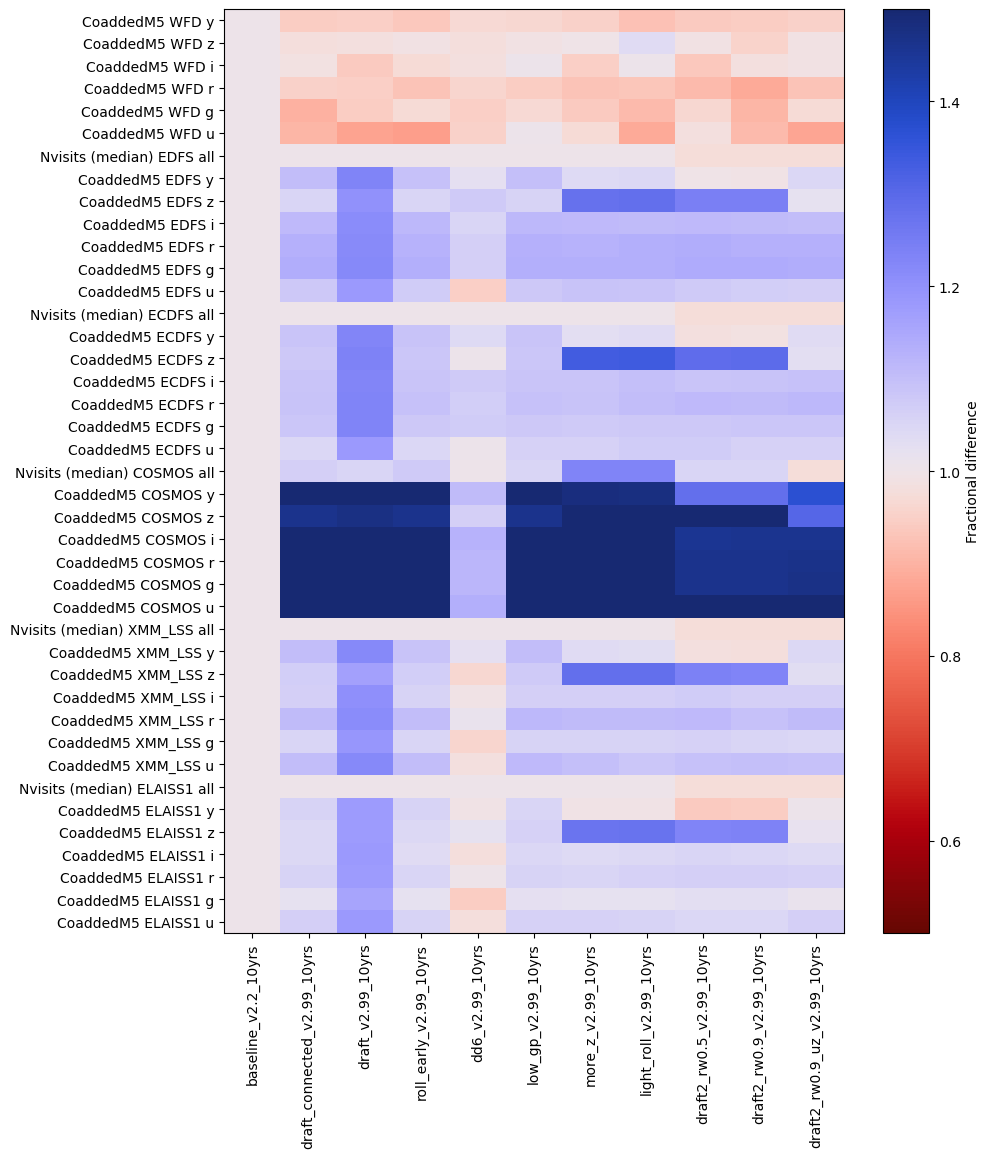
\includegraphics[width=0.6\textwidth]{figures/ddf.png}
    \caption{Coadded 10-year depth (magnitude) of the WFD and each the five DDFs that LSST will observe in each band for \texttt{baseline\_v2.2} (used as reference) and a set of v2.99 simulations. Note the increased depth for the COSMOS field, as per SCOC Phase 2 recommendation, and the inclusion of the EDFS in the final set of LSST DDFs. The filter balance in the DDFs can be tweaked, independently of the filter balance in the WFD. Note: the simulation appearing here as \texttt{draft\_rw0.9\_uz\_v2.99\_10yrs} was subsequently adopted as \texttt{baseline\_v3.0}.}
    \label{fig:my_label}
\end{figure}
